In this chapter the process of loading individual levels will be explained. This involves loading the level - encoded as an image in the PNG format -
parsing values from this format, and finally placing tiles in the game world
representing those values.

\section{Designing and loading levels}
Level creation is an important aspect when developing a game, and for this project there are different elements to consider level creation.
\begin{itemize}
    \item The development process, is an agile process, meaning the level should be easily modifiable to adapt to changes
    
    \item Game balancing, requiring the production of levels at a sufficient pace in
        order to quickly iterate on game balancing topics, such as strategies
        for a particular map layout
        
    \item The project have no dedicated level designer, that have the time
        allocated to finely tune and manually design levels
\end{itemize}
These elements sets up some different challenges to the project. 
To keep up with potential changes a fast way to create levels is preferred.
Therefore an automated process for designing levels would be desired for the following reasons:
\begin{itemize}
    \item Manually designing levels and placing gameobject in the Editor does
        not afford quick iterations, as required by our development process.
    \item The Editor does not afford easy refactoring of large levels, in that
        objects must be moved or replaced by hand. \textit{Large} is relative,
        but for our purposes it could be upwards +10.000 gameobjects.
    \item Individual levels would have to reside in individual \texttt{Scene}
        files, increasing the complexity of collaboration since scenefiles do
        not merge well in version controls.
\end{itemize}
While there are different approaches for circumventing the above inconveniences, our solution is to encode the layout of each individual level in an external file which is then loaded and interpreted. 
Historically, game developers have often used this approach, usually encoded in some in-house binary format. \todoanders{Brian, add ref here}
While customized in-house format would give more flexibility, but it would also give more work if the players should have the option to create their own levels. Because a custom level editor would be neeeded.
Instead a the choice of encoding the map in the PNG (Portable Network Graphics) was made for the following reasons:
\begin{itemize}
    \item The PNG format is ubiquitous, in that there exists support for it
        almost anywhere, including in Unity3d - both in terms of API and the
        editor itself.
    \item It being ubiquitous means that we do not have to develop additional
        software in order to edit levels - most mainstream image editors
        support the PNG format.
    \item The PNG allows us to encode \textit{enough} information.
        \textit{Enough} being relative, but each colorchannel for each
        individual pixel offers 1 \texttt{byte} of information. With each pixel
        being encoded with RGBA (red, green, blue and alpha) channels, that
        gives us a total of 4 \texttt{bytes} of information, for each pixel.
\end{itemize}
Using the PNG format, it is then only a matter of specifying \textit{what} a particular color should encode and interpreting that color when loading a level. 
As an example, the following could specify how colors could be specified to encode information about a level:
\begin{itemize}
    \item Black would be ground
    \item Green is grass
    \item Red is building floor, and
    \item Yellow being building walls.
\end{itemize}
One obvious shortcoming from the above example is the lack of variation - maybe one would like to be able to specify different types of walls or floors. This could however be mitigated by either specifying more colors or by interpreting a color differently depending on the context of the pixel.
To introduce variety into our levels, we use the latter approach for some colors, which we will describe later in this chapter.
\\

Having decided on the format and encoded color values, we can design levels such as seen in figure~\ref{fig:png_map}.

\begin{figure}[H]
    \centering
    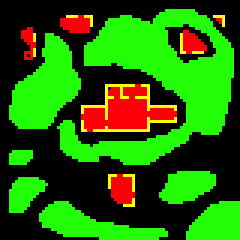
\includegraphics{figures/generating_levels/map.png}
    \caption{A PNG image encoding a level}
    \label{fig:png_map}
\end{figure}
By looking at Figure~\ref{fig:png_map}, it is illustrated that there are some patches of grass, a building in the middle of the map and some torn-down buildings in the periphery of the map encoded in the PNG.
Some individual pixels of magenta color can be seen, which encode where monster should appear. 
Likewise, a single white pixel encode the exit point of the map, which is where players are required to go to when the missions for this map have been completed. 
And last, a single blue pixels encodes where the crafting table should be placed within the level.
\\\\
The color values can then be interpreted into distinct integer values in a two-dimensional array, as seen in Figure~\ref{fig:png_to_array}.
%thread carefully below...
\begin{figure}[H]
    \centering
    \begin{tabular}{cc}
        {\footnotesize
            \setlength{\tabcolsep}{4.5pt}
            \begin{tabular}{|c|c|c|c|c|c|c|c|c|c|}
                \hline
                \cellcolor{black} & \cellcolor{black} & \cellcolor{black} &
                \cellcolor{black} & \cellcolor{black} & \cellcolor{red} &
                \cellcolor{red} & \cellcolor{red} & \cellcolor{red} &
                \cellcolor{red} \\ \hline
                \cellcolor{green} & \cellcolor{green} & \cellcolor{black} &
                \cellcolor{black} & \cellcolor{black} & \cellcolor{yellow} &
                \cellcolor{red} & \cellcolor{red} & \cellcolor{red} &
                \cellcolor{red} \\ \hline
                \cellcolor{green} & \cellcolor{green} & \cellcolor{green} &
                \cellcolor{black} & \cellcolor{black} & \cellcolor{yellow} &
                \cellcolor{red} & \cellcolor{red} & \cellcolor{red} &
                \cellcolor{red} \\ \hline
                \cellcolor{green} & \cellcolor{green} & \cellcolor{green} &
                \cellcolor{black} & \cellcolor{black} & \cellcolor{yellow} &
                \cellcolor{red} & \cellcolor{red} & \cellcolor{red} &
                \cellcolor{red} \\ \hline
                \cellcolor{green} & \cellcolor{green} & \cellcolor{green} &
                \cellcolor{black} & \cellcolor{black} & \cellcolor{yellow} &
                \cellcolor{yellow} & \cellcolor{red} & \cellcolor{red} &
                \cellcolor{yellow} \\ \hline
                \cellcolor{green} & \cellcolor{green} & \cellcolor{green} &
                \cellcolor{black} & \cellcolor{black} & \cellcolor{black} &
                \cellcolor{black} & \cellcolor{black} & \cellcolor{black} &
                \cellcolor{black} \\ \hline
                \cellcolor{green} & \cellcolor{green} & \cellcolor{green} &
                \cellcolor{green} & \cellcolor{black} & \cellcolor{black} &
                \cellcolor{black} & \cellcolor{black} & \cellcolor{black} &
                \cellcolor{black} \\ \hline
                \cellcolor{green} & \cellcolor{green} & \cellcolor{green} &
                \cellcolor{green} & \cellcolor{black} & \cellcolor{black} &
                \cellcolor{black} & \cellcolor{black} & \cellcolor{black} &
                \cellcolor{black} \\ \hline
                \cellcolor{green} & \cellcolor{green} & \cellcolor{green} &
                \cellcolor{green} & \cellcolor{green} & \cellcolor{black} &
                \cellcolor{black} & \cellcolor{black} & \cellcolor{black} &
                \cellcolor{black} \\ \hline
                \cellcolor{green} & \cellcolor{green} & \cellcolor{green} &
                \cellcolor{green} & \cellcolor{green} & \cellcolor{green} &
                \cellcolor{green} & \cellcolor{green} & \cellcolor{green} &
                \cellcolor{black} \\ \hline
            \end{tabular}
        }
        &
        {\footnotesize
            \setlength{\tabcolsep}{2.5pt}
            \begin{tabular}{|c|c|c|c|c|c|c|c|c|c|}
                \hline
                0 & 0 & 0 & 0 & 0 & 4 & 4 & 4 & 4 & 4 \\ \hline
                1 & 1 & 0 & 0 & 0 & 3 & 4 & 4 & 4 & 4 \\ \hline
                1 & 1 & 1 & 0 & 0 & 3 & 4 & 4 & 4 & 4 \\ \hline
                1 & 1 & 1 & 0 & 0 & 3 & 4 & 4 & 4 & 4 \\ \hline
                1 & 1 & 1 & 0 & 0 & 3 & 3 & 4 & 4 & 3 \\ \hline
                1 & 1 & 1 & 0 & 0 & 0 & 0 & 0 & 0 & 0 \\ \hline
                1 & 1 & 1 & 1 & 0 & 0 & 0 & 0 & 0 & 0 \\ \hline
                1 & 1 & 1 & 1 & 0 & 0 & 0 & 0 & 0 & 0 \\ \hline
                1 & 1 & 1 & 1 & 1 & 0 & 0 & 0 & 0 & 0 \\ \hline
                1 & 1 & 1 & 1 & 1 & 1 & 1 & 1 & 1 & 0 \\ \hline
            \end{tabular}
        }
    \end{tabular}
    \caption{Interpreting a PNG map image into a two-dimensional array}\label{fig:png_to_array} 
\end{figure}
Values are then further separated into a new two-dimensional array consisting of only each individual value, as illustrated on the right side in Figure \ref{fig:png_to_array}.  
The data within those arrays are what we use to generate tiles and some game entities within the gameworld.

\section{Generating level backdrop}
As explained previously, our game is a top-down 2D action game. Important to
note is the top-down 2D aspect of it when we are to generate our levels.
A historical and still prevalent technique for 2D games, is using a
tiling approach for the layout of both the backdrop of the level and entities
within it. Several different approaches to tiling have been used in games,
including squares, isometric and hexagonal tiles.
Figures~\ref{fig:civ-1_square},~\ref{fig:civ-2_iso}~and~\ref{fig:wesnoth_hex}
show examples of games using each of the mentioned techniques of
tiling.

\begin{figure}[H]
    \centering
    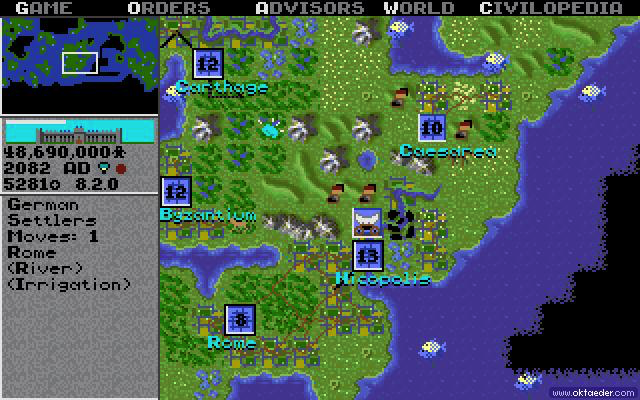
\includegraphics[scale=0.4]{figures/generating_levels/civ-1_square.png}
    \caption{Civilizations 1, using squares as tiles}\label{fig:civ-1_square} 
\end{figure}

\begin{figure}[H]
    \centering
    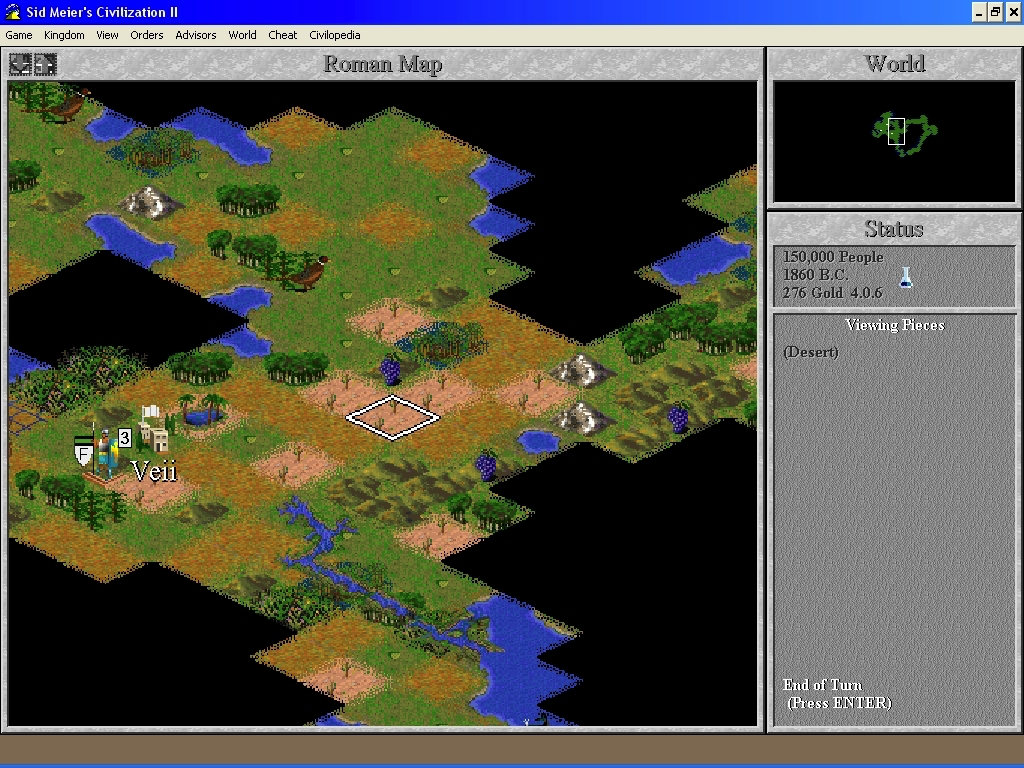
\includegraphics[scale=0.4]{figures/generating_levels/civ-2_iso.png}
    \caption{Civilizations 2, using the isometric technique}\label{fig:civ-2_iso} 
\end{figure}

\begin{figure}[H]
    \centering
    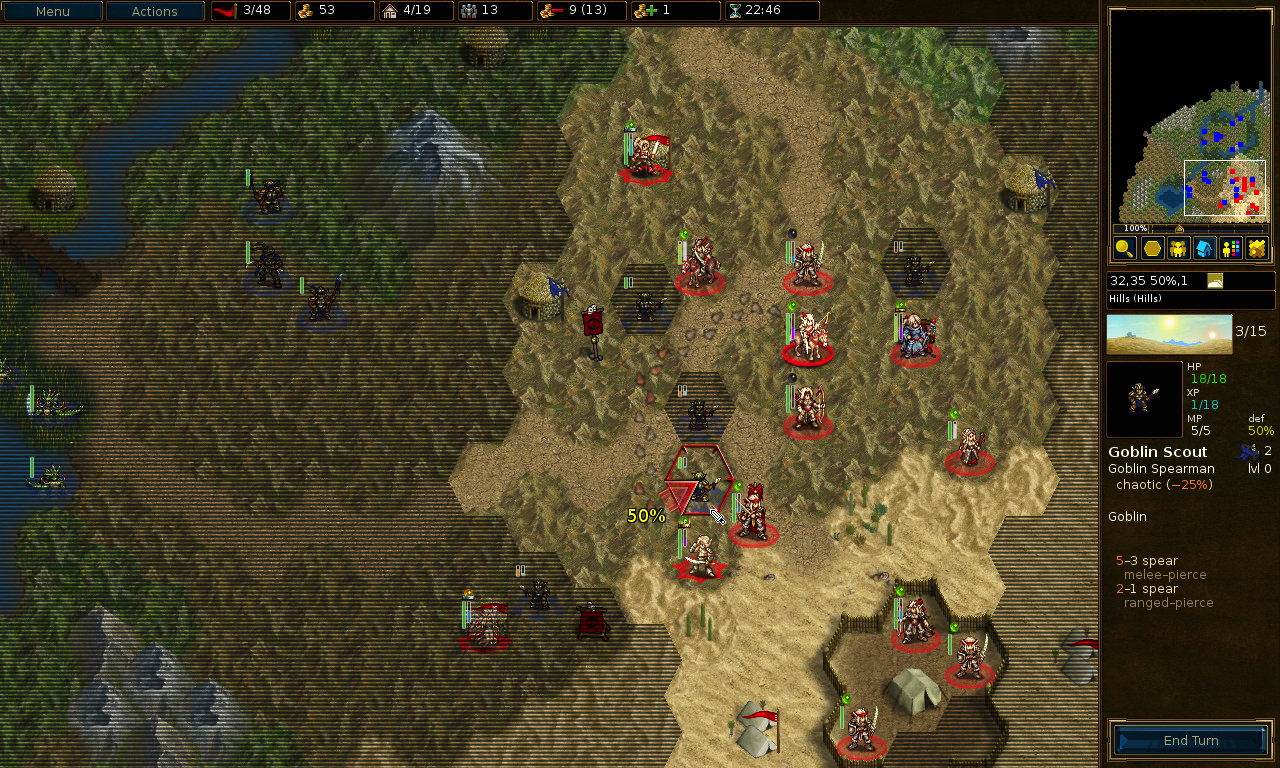
\includegraphics[scale=0.4]{figures/generating_levels/wesnoth_hex.png}
    \caption{Battle of Wesnoth, using a hexagonal tiling technique}\label{fig:wesnoth_hex} 
\end{figure}
Since the individual techniques mostly impact the visual appearance of the game, the underlying data structures remain the same.
We have chosen the apply the most straightforward tiling technique: square tiles.
\\
\\
The first naive implementation that we prototyped, was to iterate through the two-dimensional map and place tiles corresponding to the values, with tiles
being \texttt{sprites} in the gameworld. 
In Unity sprites needs to be assigned a \texttt{sprite renderer} component which in turn needs to be attached a \texttt{gameobject}. 
This effectively means that for each tile an instantiation a gameobject has to be made, which easily can get expensive in computation.

Since tiles exhibit no particular behaviour, it seems excessive to instantiate gameobjects for each tile. 
Not only that, but we were experiencing performance implications on mobile devices using this method.  
It is possible to substantially reduce the gameobjects required to be instantiated by \textit{grouping} similar areas into bigger tiles. 
To do the map needs to be grouped such that large area consisting of only one type will be marked.
The groups then \textit{blit} the texture associated with that type in a tile-pattern, onto a bigger texture.  
There is a technical limit to this technique however, as texture-resolutions are limited by hardware. 
For our particular implementation, we limit the resolution to 1024x1024 pixels, which is within the limits of our target hardware. 
A comparison of the result of the two techniques can be seen in figure~\ref{fig:grouped_tiling_comparison}.
\begin{figure}[H]
    \centering
    \begin{tabular}{cc}
        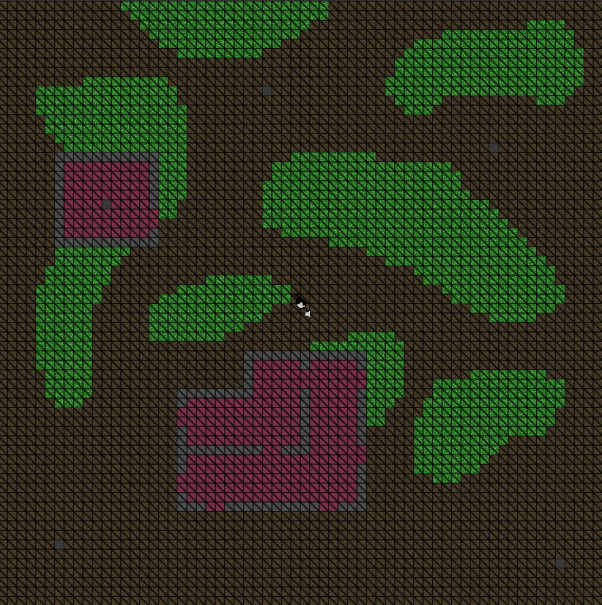
\includegraphics[width=0.5\textwidth]{figures/generating_levels/naive-tile.png}
        &
        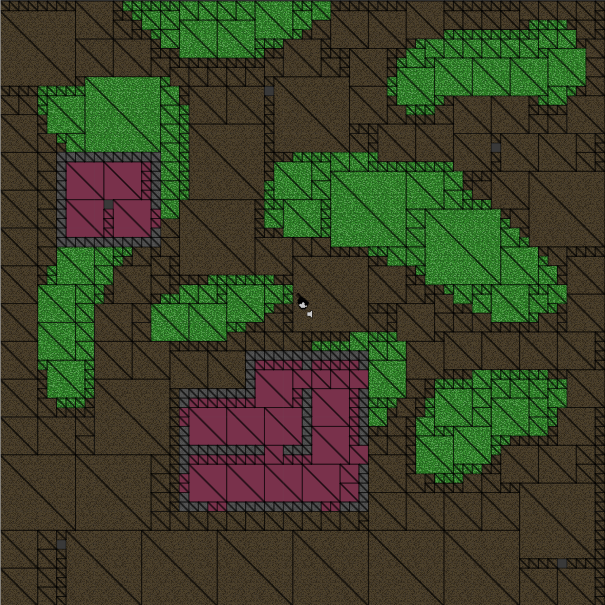
\includegraphics[width=0.5\textwidth]{figures/generating_levels/grouped-tile.png}
    \end{tabular}
    \caption{(left) naive tiling, (right) grouping tiles into larger tiles}\label{fig:grouped_tiling_comparison}
\end{figure}
The blitting is performed during runtime whenever a map is loaded, but in order to avoid blitting the same texture more than once, a caching of the larger tiles to disk such that they can be loaded between subsequent runs of the application. 
The performance overhead of blitting \textit{can} be significant on mobile devices, as the larger textures have to be uploaded to the GPU in order to reflect changes, and we did see improvements in that regard by caching the blitted textures.
\\
\\
It is also wanted \textit{transition} tiles between certain type of tiles, in particular between grass and ground.
This technique is also used in the games seen in figures~\ref{fig:civ-1_square},~\ref{fig:civ-2_iso}~and~\ref{fig:wesnoth_hex}.
To achieve this an adaptation of the \textit{Marching squares} algorithm is used, and marks a position in the map as a particular type, based on the values  of its neighbours. 
A corresponding \textit{transition tile} is then blitted together (and cached to disk in the same manner as grouped tiles), and assigned to it.
Figure~\ref{fig:transition_comparison} shows a comparison before and after integrating the algorithm.
\todobrian{add ref for marching squares}

\begin{figure}[H]
    \centering
    \begin{tabular}{cc}
        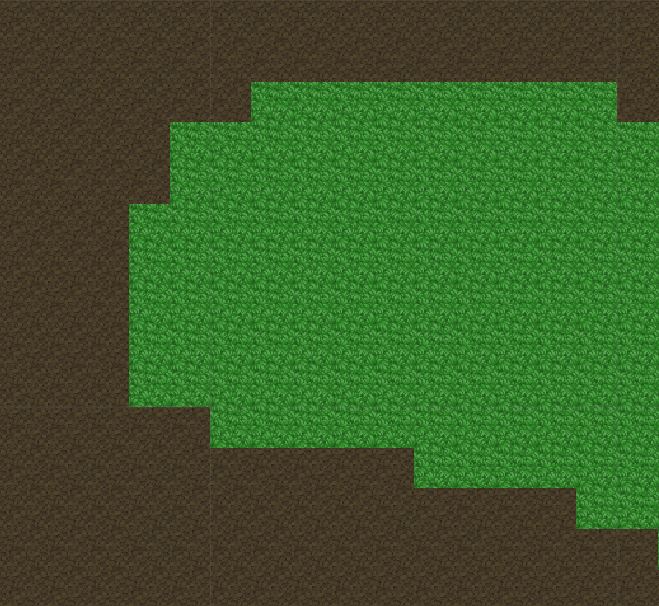
\includegraphics[width=0.5\textwidth]{figures/generating_levels/no_transition.png}
        &
        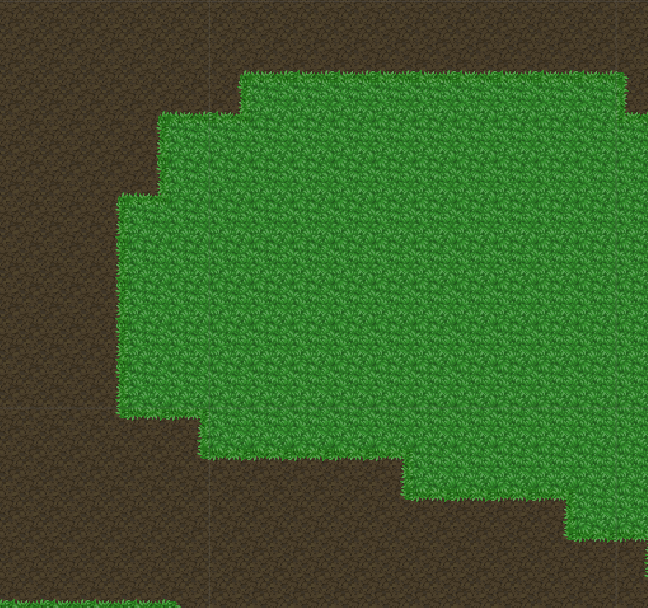
\includegraphics[width=0.5\textwidth]{figures/generating_levels/with_transition.png}
    \end{tabular}
    \caption{(left) without transitioning, (right) with transitioning tiles}\label{fig:transition_comparison}
\end{figure}

\section{Placing walls and colliders}
Placing walls involves both placing them as textured tiles within the gameworld, and placing \textit{colliders} such that moving object in the game cannot move through them.

\subsection{Placing wall sprites}
A naive implementation for placing wall sprites within the gameworld is to place
a gameobject with the texture of a wall. However, the walls should look
``connected'' as if constructed together as on homogeneous unit. This is done
using an adaptation of the \textit{Marching squares}, following the same procedure as with
transitional tiles between grass and ground. Firstly it is detected if a wall is a
``stump'', a regular vertical or horizontal middle section or a t-section. 
Diagonal wall are treated as ''stumps'', so our marching squares adaptation only
considers adjacent tiles at 90-degree angles. Figure~\ref{fig:wall_comparison}
illustrates an example of placing walls where tiles are ``connected'' and one where
tiles are ``connected'' and figure~\ref{fig:walls_ingame} showing an in-game
example.

\begin{figure}[H]
    \centering
    \begin{tabular}{cc}
        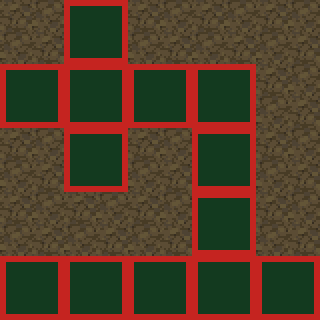
\includegraphics[width=0.5\textwidth]{figures/generating_levels/wall_no_border.png}
        &
        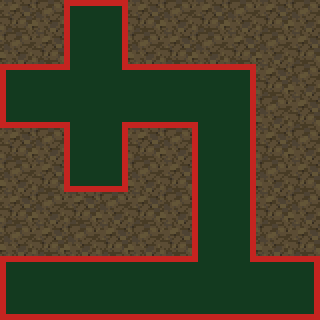
\includegraphics[width=0.5\textwidth]{figures/generating_levels/wall_with_border.png}
    \end{tabular}
    \caption{(left) not connected, and (right) where walls are connected}\label{fig:wall_comparison}
\end{figure}

\begin{figure}[H]
    \centering
    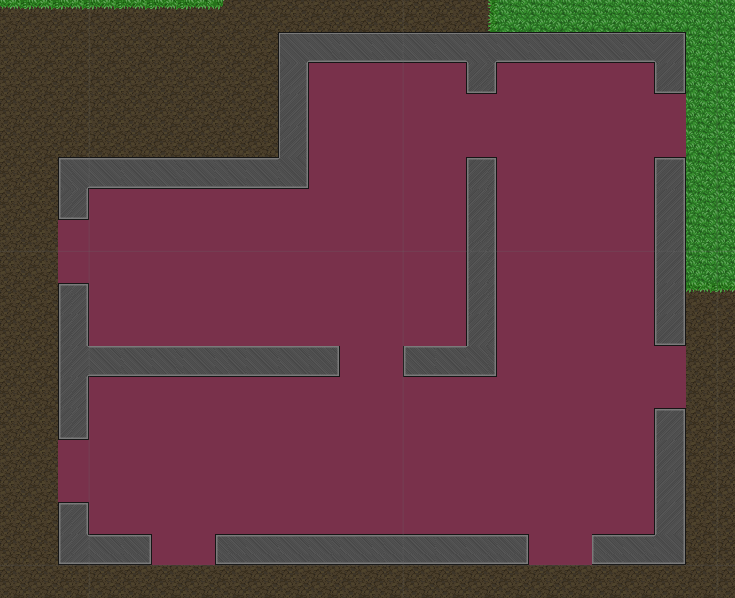
\includegraphics[width=1\textwidth]{figures/generating_levels/walls_ingame.png}
    \caption{In-game example of connected walls}\label{fig:walls_ingame} 
\end{figure}

\subsection{Placing wall colliders}
For wall colliders it is desired to \textit{translate} the contour of walls into
gameobjects assigned a collide-able component in the gameworld. The first naive
implementation is to was to place a square collider (regular
\texttt{Collider2D}) for each wall tile.
The positions for these colliders is shown as red dots in
figure~\ref{fig:wall_with_vertices}.
This resulted in the unfortunate behaviour that collisions from rigidbodies -
the player and enemies - behaved unreliable and rigid bodies would ``bounce off''
the walls whenever they would be ``between'' two collider sections.
\\
The next idea is to find offsets for countour vertices for each tile, and
placing \texttt{Polygon Collider2D}, contour vertices shown as blue in
figure~\ref{fig:wall_with_vertices}. However this reveals another problem: the resulting
polygon is concave. This means that the polygon cannot
\textit{easily} be constructed only knowing the vertices. Our
solution was to use an adaptation of \textit{flood fill} to first find
connected vertical and then horizontal wall sections. From the algorithm, we
can find vertices for and construct concave polygons which are \textit{larger}
than single wall sections. This significantly reduces the number of colliders
necessary, almost eliminates the mentioned problem of unreliable behavior for
rigid bodies colliding with walls. An \textit{optimal} solution would be to
construct a concave polygon from the vertices, which would require finding all
countour vertices \textit{and} the order in which they should connected when
constructing the polygon. The result of our \textit{flood fill} approach can be
seen in figure~\ref{fig:wall_with_convex}.

\begin{figure}[H]
    \centering
    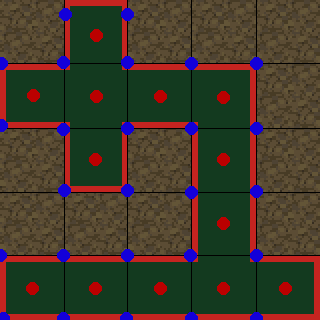
\includegraphics[width=1\textwidth]{figures/generating_levels/wall_with_vertices.png}
    \caption{Finding contour vertices}\label{fig:wall_with_vertices} 
\end{figure}

\begin{figure}[H]
    \centering
    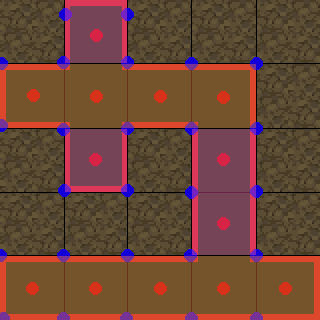
\includegraphics[width=1\textwidth]{figures/generating_levels/wall_with_convex.png}
    \caption{Finding connected concave polygons using flood fill}\label{fig:wall_with_convex} 
\end{figure}
